\documentclass[12pt]{article}
\usepackage[utf8]{inputenc}
\usepackage[italian]{babel}
\usepackage{circuitikz}
\usepackage{float}
\usepackage{mathptmx}
\usepackage{graphicx}
\usepackage{subcaption}
\usepackage{nicefrac}
\usepackage[a4paper, top=2cm, bottom=1.5cm, left=2cm, right=2cm]{geometry}

\title{Analisi di un Filtro Crossover} 
\author{Samuele Lanzi mat. 941813}
\date{7 Aprile, 5 Maggio, 26 Maggio 2021}

\begin{document}
\maketitle
%\renewcommand{\theequation}{\thesection.\arabic{equation}}
\section{Sommario}
L'esperienza svolta ha permesso di analizzare il comportamento di un filtro crossover sottoposto a differenti 
segnali in entrata. Acquisendo i dati relativi ai due rami del circuito al variare della frequenza del segnale è stato possibile stimare
la frequenza di crossover tipica del circuito. Dapprima è stata analizzata l'ampiezza del segnale in funzione della frequenza portando 
risultati positivi in quanto la stima della frequenza di crossover $\nu_0 = (4024 \pm 4) \ Hz$ è risultata compatibile 
con quella attesa di valore $\nu_0 = (4021 \pm 40) \ Hz$. Dopodiché è stato analizzato lo sfasamento della tensione 
nei rami rispetto a quella generata, che ha portato ad una misura indipendente della frequenza di crossover pari a $\nu_0=(4007\pm 16) \ Hz$ 
anch'essa compatibile con quella attesa.

\section{Introduzione}
Il filtro crossover è un tipo di circuito utilizzato nei sistemi di riproduzione audio
allo scopo di dividere il segnale in due range di frequenze associati a due speakers: 
\textit{tweeter} per alte frequenze e \textit{woofer} per basse frequenze. Uno schema 
del circuito realizzato è rappresentato in Fig. \ref{Fig1}. I componenti 
di un filtro crossover passivo sono induttanze, condensatori e resistori 
ed i rami costituiscono un filtro passa-basso ed un filtro passa-alto. La frequenza di separazione del 
se\nu_0=\frac{1}{2\pi\sqrt{LC}}=\frac{1}{2\pi\sqrt{\tau_L\tau_C}}gnale è specifica del circuito e viene detta \textit{frequenza di crossover}; si dimostra 
(dettagli in appendice) che tale frequenza è determinata da
\begin{equation}
  
\end{equation} 
\
\\
con $\tau_L = \nicefrac{L}{(R_L + R_{IL})}$ e $\tau_C = (R_C+R_{IC}) C$ rispettivamente tempi caratteristici del filtro passa-basso
e filtro passa-alto.
Applicando in input una tensione sinusoidale di frequenza fissata ed ampiezza costante ci si aspetta di rilevare ai capi delle resistenze
$R_L$ ed $R_C$ due segnali alla stessa frequenza di entrata ma di ampiezza diversa dipendente dalla frequenza. D'atra parte studiando lo sfasamento
ci si aspetta un andamento decrescente all'aumentare della frequenza in entrambi i rami. Si può quindi estrapolare sperimentalmente la frequenza di crossover osservando per quale valore della frequenza in ingresso si ha 
la stessa ampiezza oppure uno sfasamento opposto sui due rami. %Se al circuito viene applicata in entrata un'onda quadra i due 
%rami del circuito si comporteranno come un circuito RL in evoluzione libera e come un circuito RC nella fase scarica e, anche in
%questo caso è possibile ricavarsi i tempi caratteristici dei rami al fine di stimare la frequenza di crossover.
% Figure 1 %%%%%%%%%%%%%%%%%%%%%%%%%%%%%%%%

%%%%%%%%%%%%%%%%%%%%%%%%%%%%%%%%%%%%%%%%%%%

\section{Apparato Sperimentale}
Il circuito in Fig. \ref{Fig1} è stato assemblato sulla breadboard della scheda di acquisizione dati NI ELVIS II. I due rami del circuito sono collegati
al \textit{Function Generator} (FGEN) di ELVIS avente resistenza interna $R_\varepsilon = 50 \ \Omega$. Sul ramo del woofer sono presenti un'induttanza di 
valore $L=(47.2 \pm 0.5) \ mH$ avente resistenza interna $R_{IL}=(198.8\pm0.5) \ \Omega$ ed una resistenza collegata in serie $R_L=(994\pm5) \ \Omega$;
in parallelo, sul ramo del tweeter, sono presenti un condensatore di capacità $C=(33.2\pm0.3) \ nF$ e due resistenze in serie $R_C=(993\pm5) \ \Omega$ e
$R_{IC}=(201\pm1) \ \Omega$ aggiunta per compensare la resistenza interna dell'induttanza. I valori delle componenti del circuito sono stati misurati 
mediante il \textit{Digital Multimeter} di ELVIS attribuendo a tali valori le incertezze suggerite dalle specifiche della scheda di acquisizione fornite 
dal costruttore. 

Per determinare la frequenza di crossover sono stati acquisiti dati relativi alla tensione in ingresso FGEN e le tensioni ai capi di $R_L$ ed $R_C$ al 
variare della frequenza in input; quest'ultima è stata fatta variare nel range $1 \ kHz - 10 \ kHz$ con incrementi di $10 \ Hz$. L'ampiezza e la fase, 
entrambe funzioni della frequenza, sono state estrapolate da ogni acquisizione grazie al subVI \textit{Extract Single Tone Information} di LabVIEW. 
L'acquisizione è stata effettuata ad una frequenza di campionamento pari a $200 \ kHz$, grazie alla quale è stato possibile avere un grande numero di punti.
%Analizzando il circuito in regime di onda quadra alla frequenza di $1 \ kHz$ ed acquisendo lo stesso tipo di dati è stato possibile ricavare le curve caratteristiche 
%dei due rami al fine di stimare in maniera differente $\nu_0$.

\section{Risultati e Discussione}
\subsection{Analisi preliminare}
Per verificare il corretto funzionamento del filtro è stata effettuata un'analisi preliminare: in Fig. 2 sono rappresentati alcuni comportamenti del filtro al variare di FGEN, in particolare
oltre alla frequenza è stata variata anche la forma d'onda del segnale in entrata con l'ausilio dell'\textit{Arbitrary Wave Function Generator} di ELVIS. Da questa prima analisi 
è possibile notare come a basse frequenze (inferiori a quella di crossover) si rileva un'ampiezza
superiore sul ramo del woofer rispetto a quello del tweeter, ad alte frequenze si osserva il 
comportamento opposto ed alla frequenza prossima a quella di crossover le ampiezze sui due rami sono molto simili.

% Figure 2 %%%%%%%%%%%%%%%%%%%%%%%%%%%%%%%%
\begin{figure}[!ht]
  \begin{subfigure}{.5\textwidth}
    \centering
    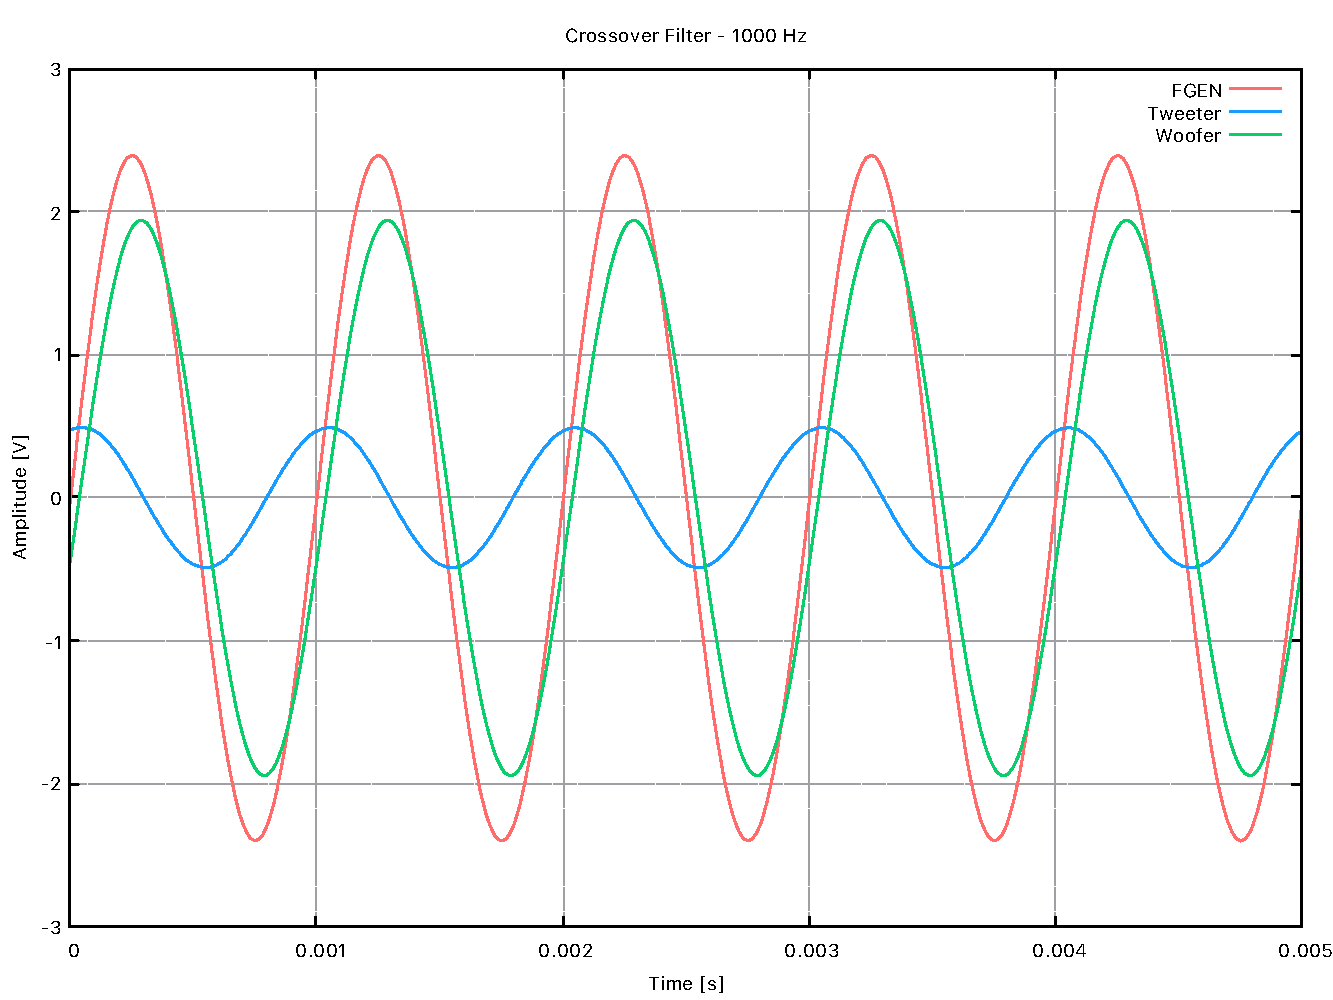
\includegraphics[width=1\linewidth]{../results/CF1000Hz.pdf}
    \caption{\textit{Comportamento del filtro a 1000 Hz
    }}
  \end{subfigure}%
  \hfill
  \begin{subfigure}{.5\textwidth}
    \centering
    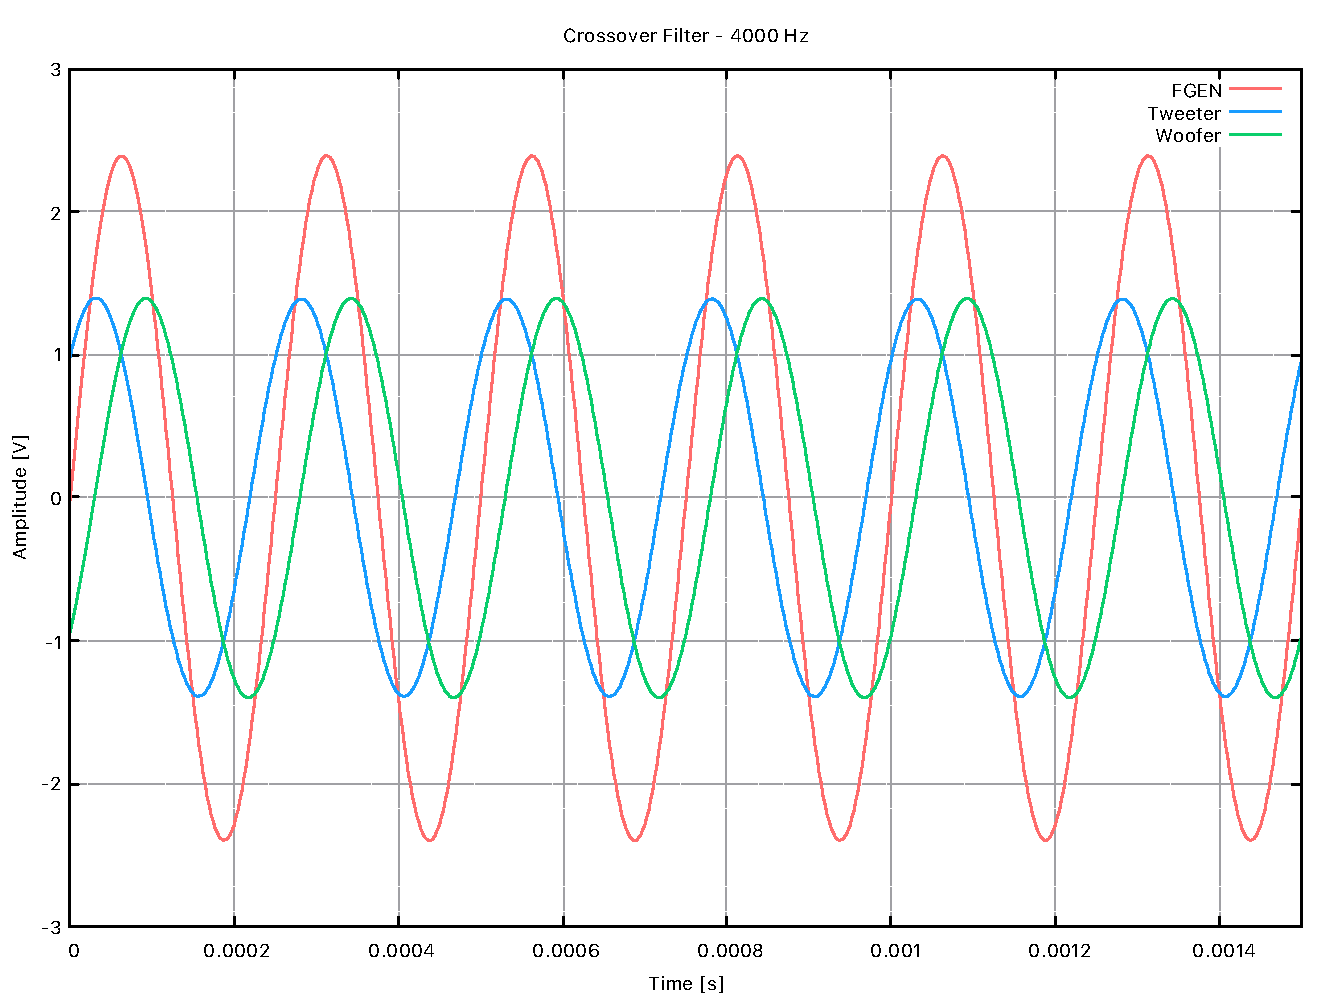
\includegraphics[width=1\linewidth]{../results/CF4000Hz.pdf}
    \caption{\textit{Comportamento del filtro a 4000 Hz}}
  \end{subfigure}
\color{white}{hdjdjfhjdhdjhfjdhfjdjfhjj}
  \begin{subfigure}{.5\textwidth}
    \centering
    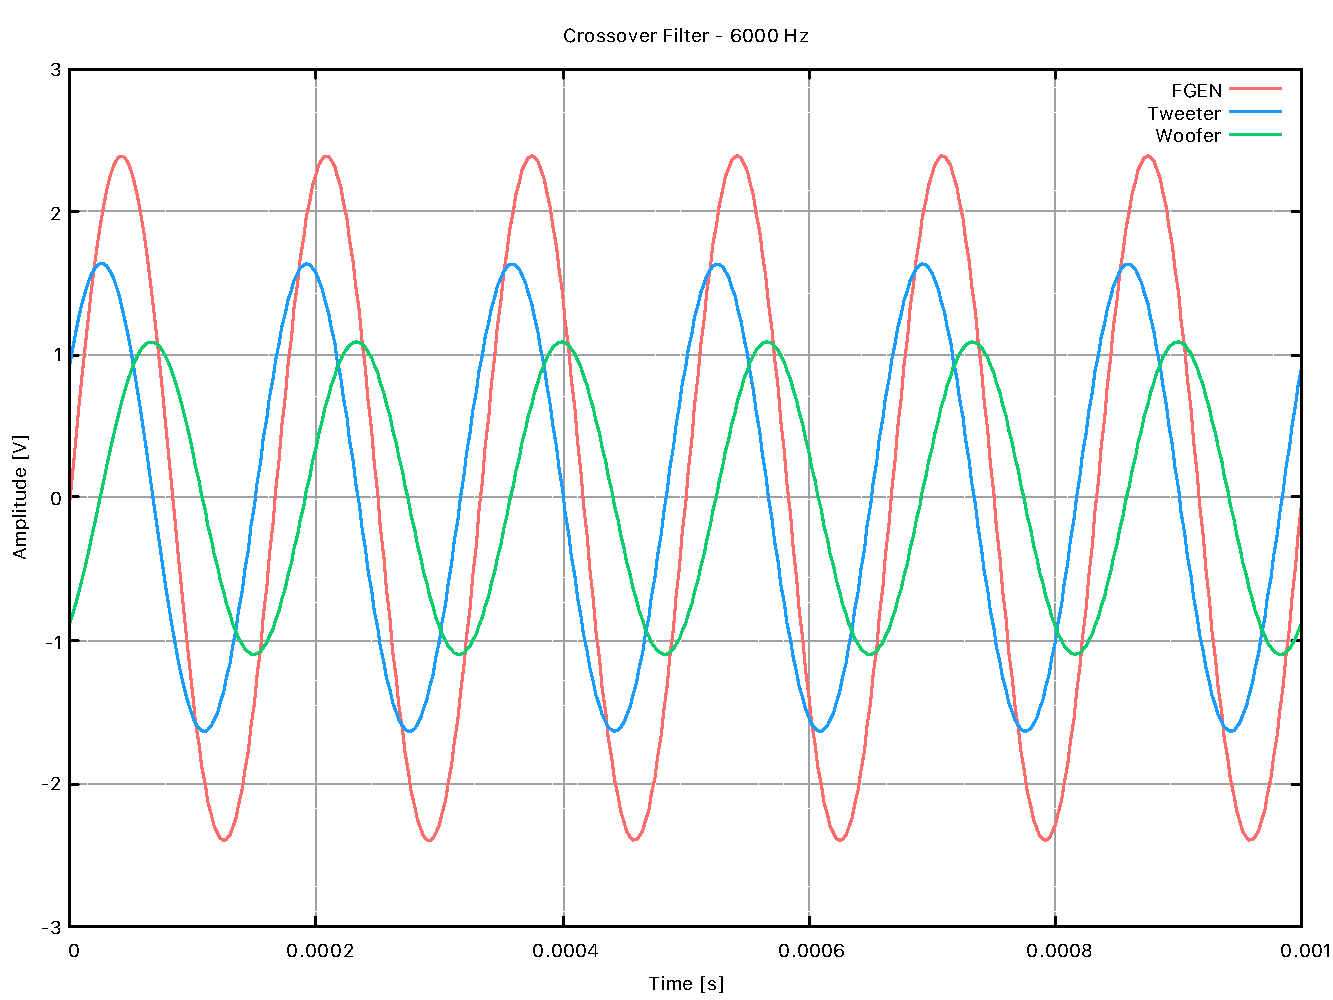
\includegraphics[width=1\linewidth]{../results/CF6000Hz.pdf}
    \caption{\textit{Comportamento del filtro a 6000 Hz}}
  \end{subfigure}%

  \begin{subfigure}{.5\textwidth}
    \centering
    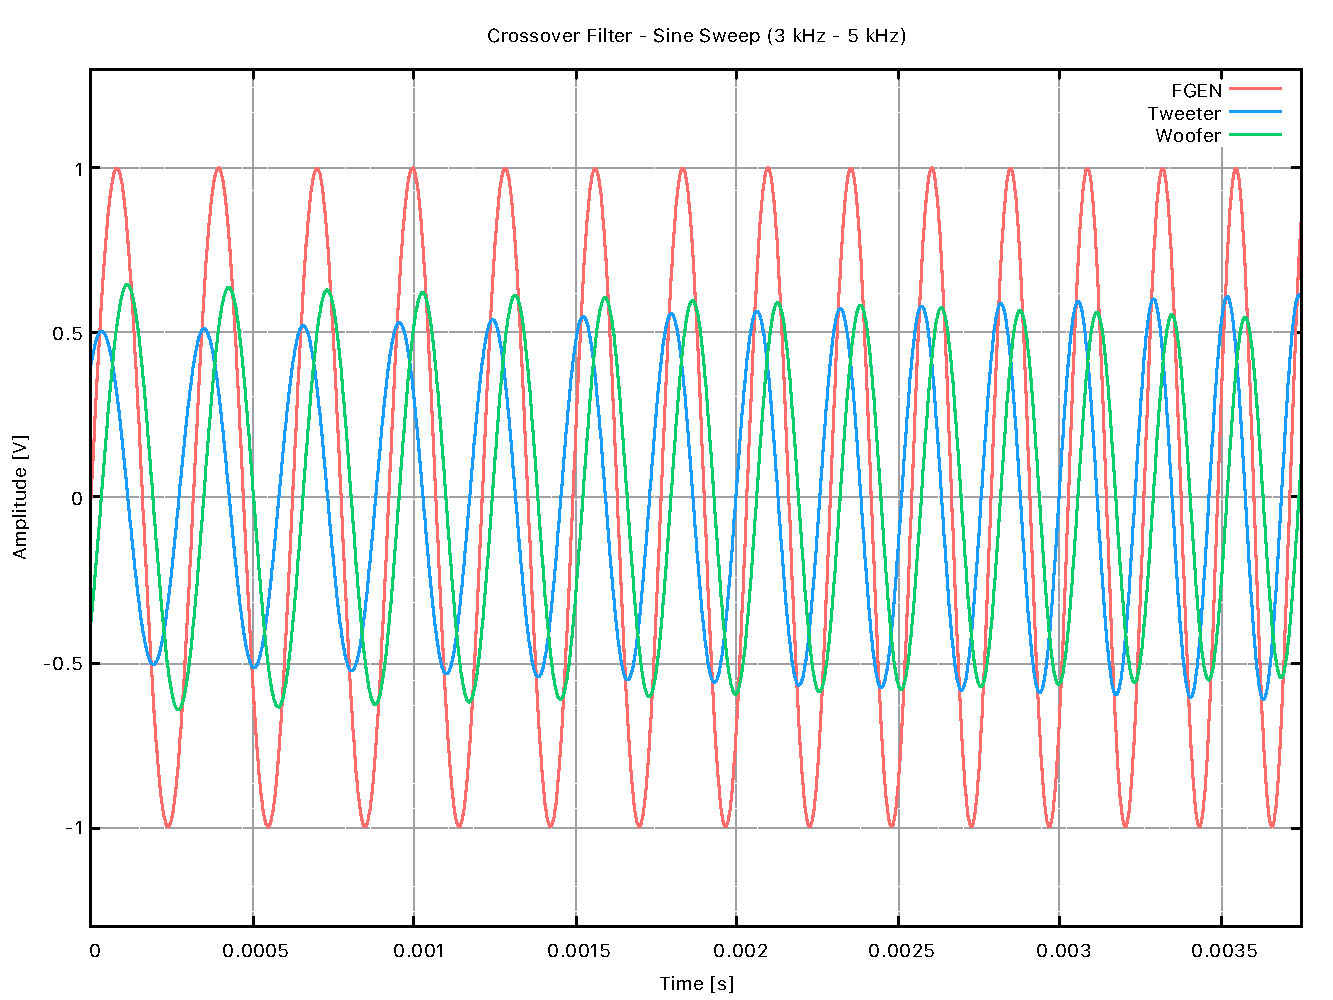
\includegraphics[width=1\linewidth]{../results/CFSineSweep.pdf}
    \caption{\textit{Comportamento del filtro sottoposto ad una Linear Sweep Sine Function. È possibile apprezzare come le ampiezze sui due rami si assomiglino tanto quanto la frequanza dell'onda si avvicini a quella di crossover.}}
  \end{subfigure}%
  \hfill
  \begin{subfigure}{.5\textwidth}
    \centering
    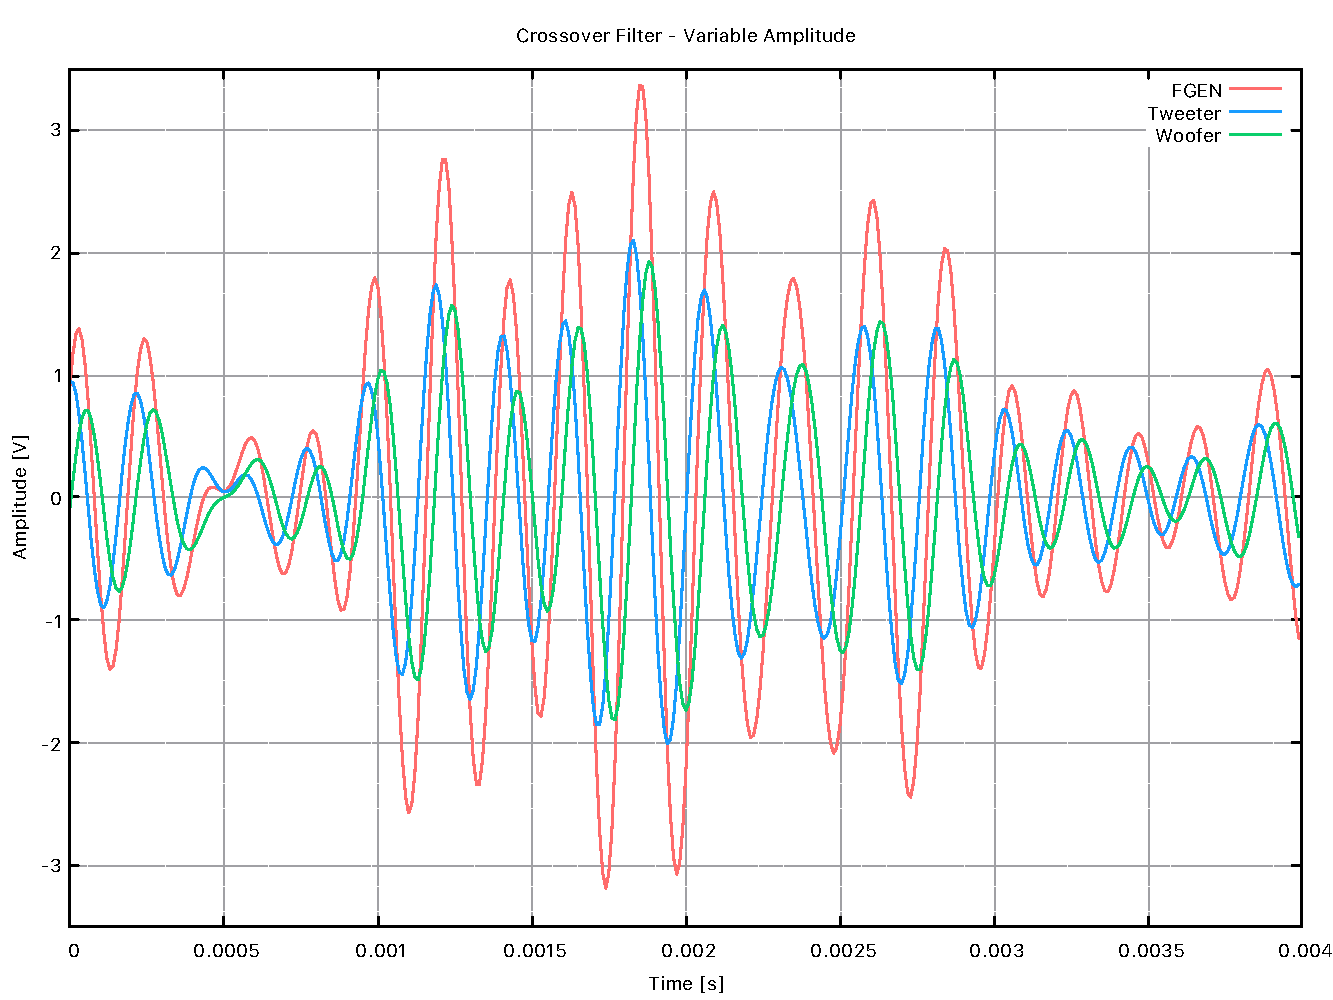
\includegraphics[width=1\linewidth]{../results/CFAmplitudeMod.pdf}
    \caption*{\centering{\textit{\ \ $(e)$ Filtro sottoposto ad un segnale 
                                di ampiezza variabile} {\color{white}{kdslfjlsdlkfslkdlsldkjfldkflskdflksdflksdflkdsfldjfksdlkfjskldsjflksdlfkjlsksldkfjlsdjklfjkslddslkfjlkdsjklfjskdl}}}}
  \end{subfigure}

  \caption{ \textit{Effetti del filtro sui vari segnali in entrata. 
  I dati sono rappresentati da linee continue a causa dei numerosi punti 
  ravvicinati.} }
\end{figure}
%%%%%%%%%%%%%%%%%%%%%%%%%%%%%%%%%%%%%%%%%%%
\newpage

\
\subsection{Analisi della tensione}
% Figure 3 %%%%%%%%%%%%%%%%%%%%%%%%%%%%%%%%
\begin{figure}[!ht]
  \begin{subfigure}{.5\textwidth}
    \centering
    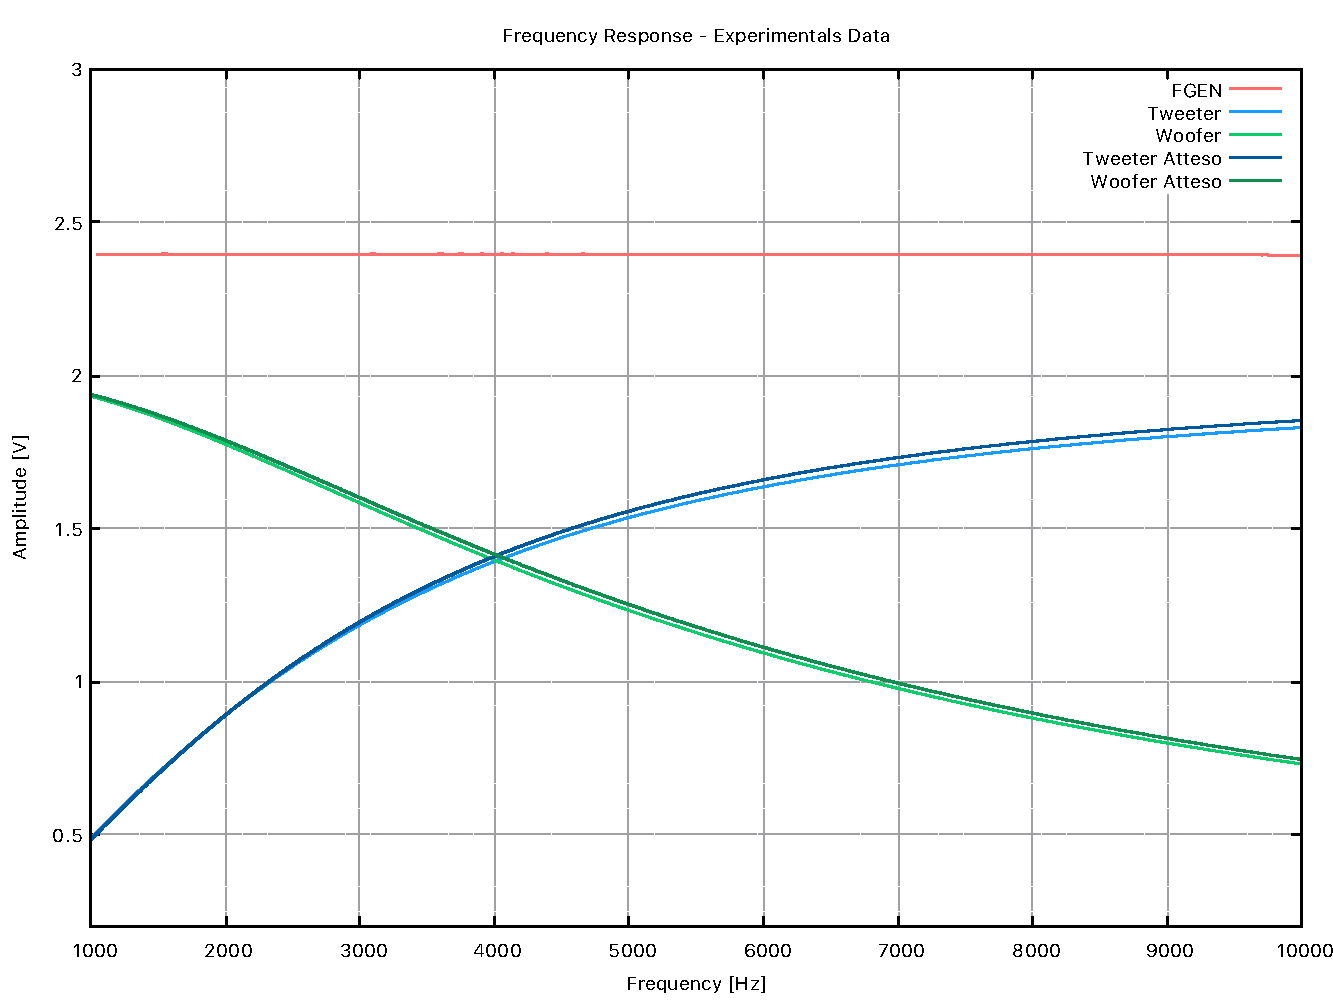
\includegraphics[width=1\linewidth]{../results/CFAmpl.pdf}
    \caption{\textit{}}
  \end{subfigure}%
  \hfill
  \begin{subfigure}{.5\textwidth}
    \centering
    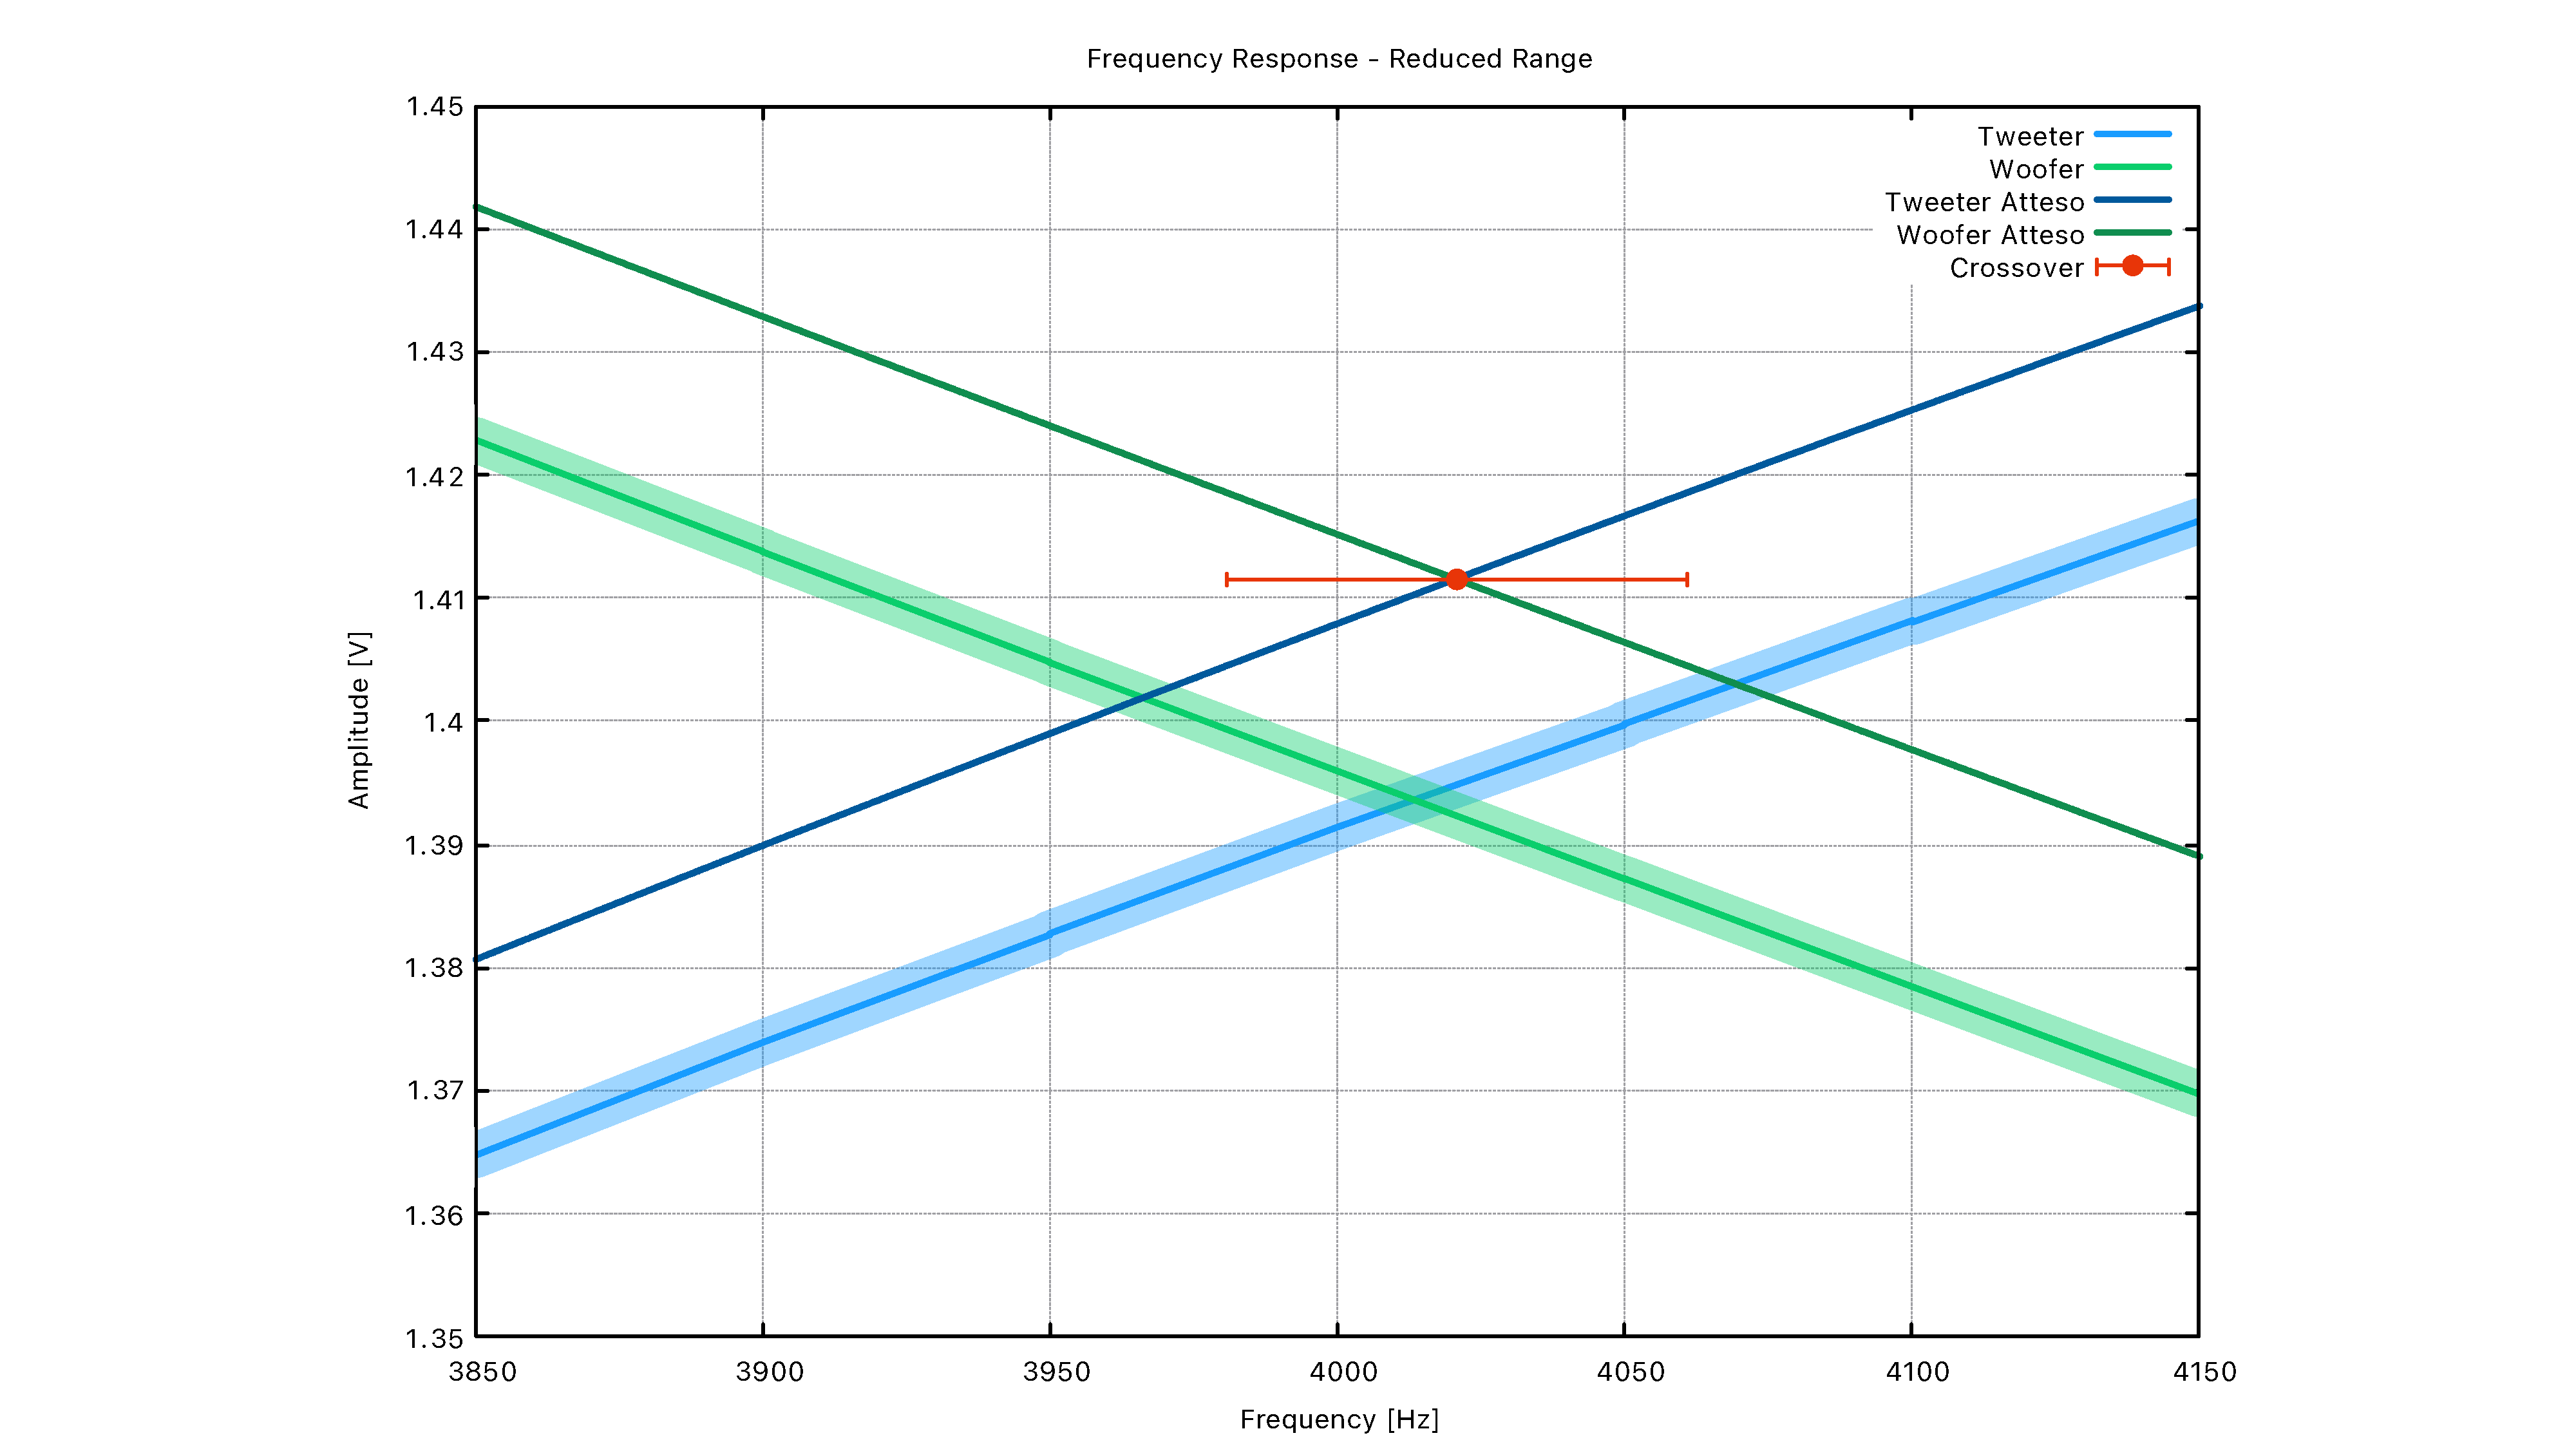
\includegraphics[width=1\linewidth]{../results/CFAmplRR.pdf}
    \caption{\textit{}}
  \end{subfigure}

  \caption{ \textit{Ampiezza del segnale rilevato in funzione della frequenza in ingresso e funzioni attese: (a) sweep effettuato tra 1 kHz e 10 kHz con step di 10Hz, (b) sweep tra 3950 Hz e 4100 Hz e valore atteso della frequenza di crossover con relativa incertezza. I dati e le incertezze sono stati rappresentati con linee e bande continue a causa dell'elevata densità di valori.} }
\end{figure}
%%%%%%%%%%%%%%%%%%%%%%%%%%%%%%%%%%%%%%%%%%%
\
\\
In Fig. 3 sono rappresentati i dati sperimentali rilevati sui rami del circuito a confronto con le curve teoriche. Ai dati sperimentali 
è stata associata un'incertezza $\delta V = 2 \ mV$ come suggerito dalle specifiche della scheda ELVIS. Le incertezze sulla frequenza sono confrontabili
con la risoluzione del \textit{Function Generator} ($0.186 \ Hz $) quindi del tutto trascurabili rispetto alle frequenze tipiche di questa esperienza.
La frequenza di crossover attesa $\nu_0=(4021 \pm 40) \ Hz$ rappresentata in Fig. 3b è stata calcolata attraverso l'equazione (1).
Gli andamenti teorici sono dati dalle seguenti espressioni:
\begin{equation}
  V_C(\nu) = V\frac{r_C}{\sqrt{1+\frac{1}{(2 \pi \tau_C \nu)^2}}} \ \ \ \ \ \ \ \ \ V_L(\nu) = V\frac{r_L}{\sqrt{1+(2 \pi \tau_L \nu)^2}}
\end{equation} $V_C$ e $V_L$ sono le ampiezze ai capi di $R_C$ ed $R_L$, $V$ la tensione in ingresso, $\nu$ la frequenza generata, $\tau_C$ e $\tau_L$ i tempi caratteristici
dei rami, $r_C=\nicefrac{R_C}{(R_C+R_{IC})}$ e $r_L=\nicefrac{R_L}{(R_C+R_{IC})}$ rappresentano i rapporti tra resistenza su cui viene misurata la tensione e la resistenza 
dell'intero ramo; per costruzione $r_C \approx r_L = 0.83 \pm 0.01$. Nella Fig. 3a notiamo che FGEN si discosta dal valore costante atteso ($2.5 \ V$) in quanto vi è una piccola
caduta di potenziale dovuta alla resistenza interna di ELVIS; tale caduta di potenziale è di circa $0.1 \ V$.

Il nostro obiettivo è quello di stimare la frequenza di crossover, quindi determinare i valori di $\tau_C$ e $\tau_L$ che meglio si adattano ai nostri dati, per fare ciò
è stato eseguito un fit delle funzioni in equazione (2) sui dati sperimentali. I risultati del fit visibili in Fig. 4 hanno fornito i parametri $\tau_C=(38.40\pm0.06) \ \mu s $ e $\tau_L=(40.27\pm0.01) \ \mu s $ 
molto vicini a quelli attesi $\tau_C=(39.6\pm0.8) \ \mu s $ e $\tau_L=(39.6\pm0.7) \ \mu s $.
I fit sono stati effettuati considerando l'ampiezza di FGEN costante e pari al suo valor medio nel range in esame, in virtù di questo fatto durante il fit è stata considerata un'incertezza sull'ampiezza 
pari alla massima distanza tra i dati relativi a FGEN ed il valor medio, ovvero $20 \ mV$. A questi fit sono associati i valori di chi quadro ridotto $\tilde{\chi^2_C}=0.44$ e $\tilde{\chi^2_L}=0.07$. Entrambi i valori
risultano inferiori al valore ottimale di 1 (soprattutto il secondo) in quanto la funzione di fit è molto vicina ai dati sperimentali rispetto all'incertezza associata (probabilmente è stata sovrastimata l'incertezza).
Utilizzando l'equazione (1) è possibile ricavare la miglior stima della frequenza di crossover $\nu_0=(4024 \pm 4) \ Hz$ visibile nel grafico in Fig. 4b; questa stima è compatibile con il valore atteso. Il valore della frequenza 
risulta molto preciso con un'incertezza percentuale del $0.1\%$, inferiore a quella associata al valore teorico.
% Figure 4 %%%%%%%%%%%%%%%%%%%%%%%%%%%%%%%%
\begin{figure}[!ht]
\begin{subfigure}{.5\textwidth}
  \centering
  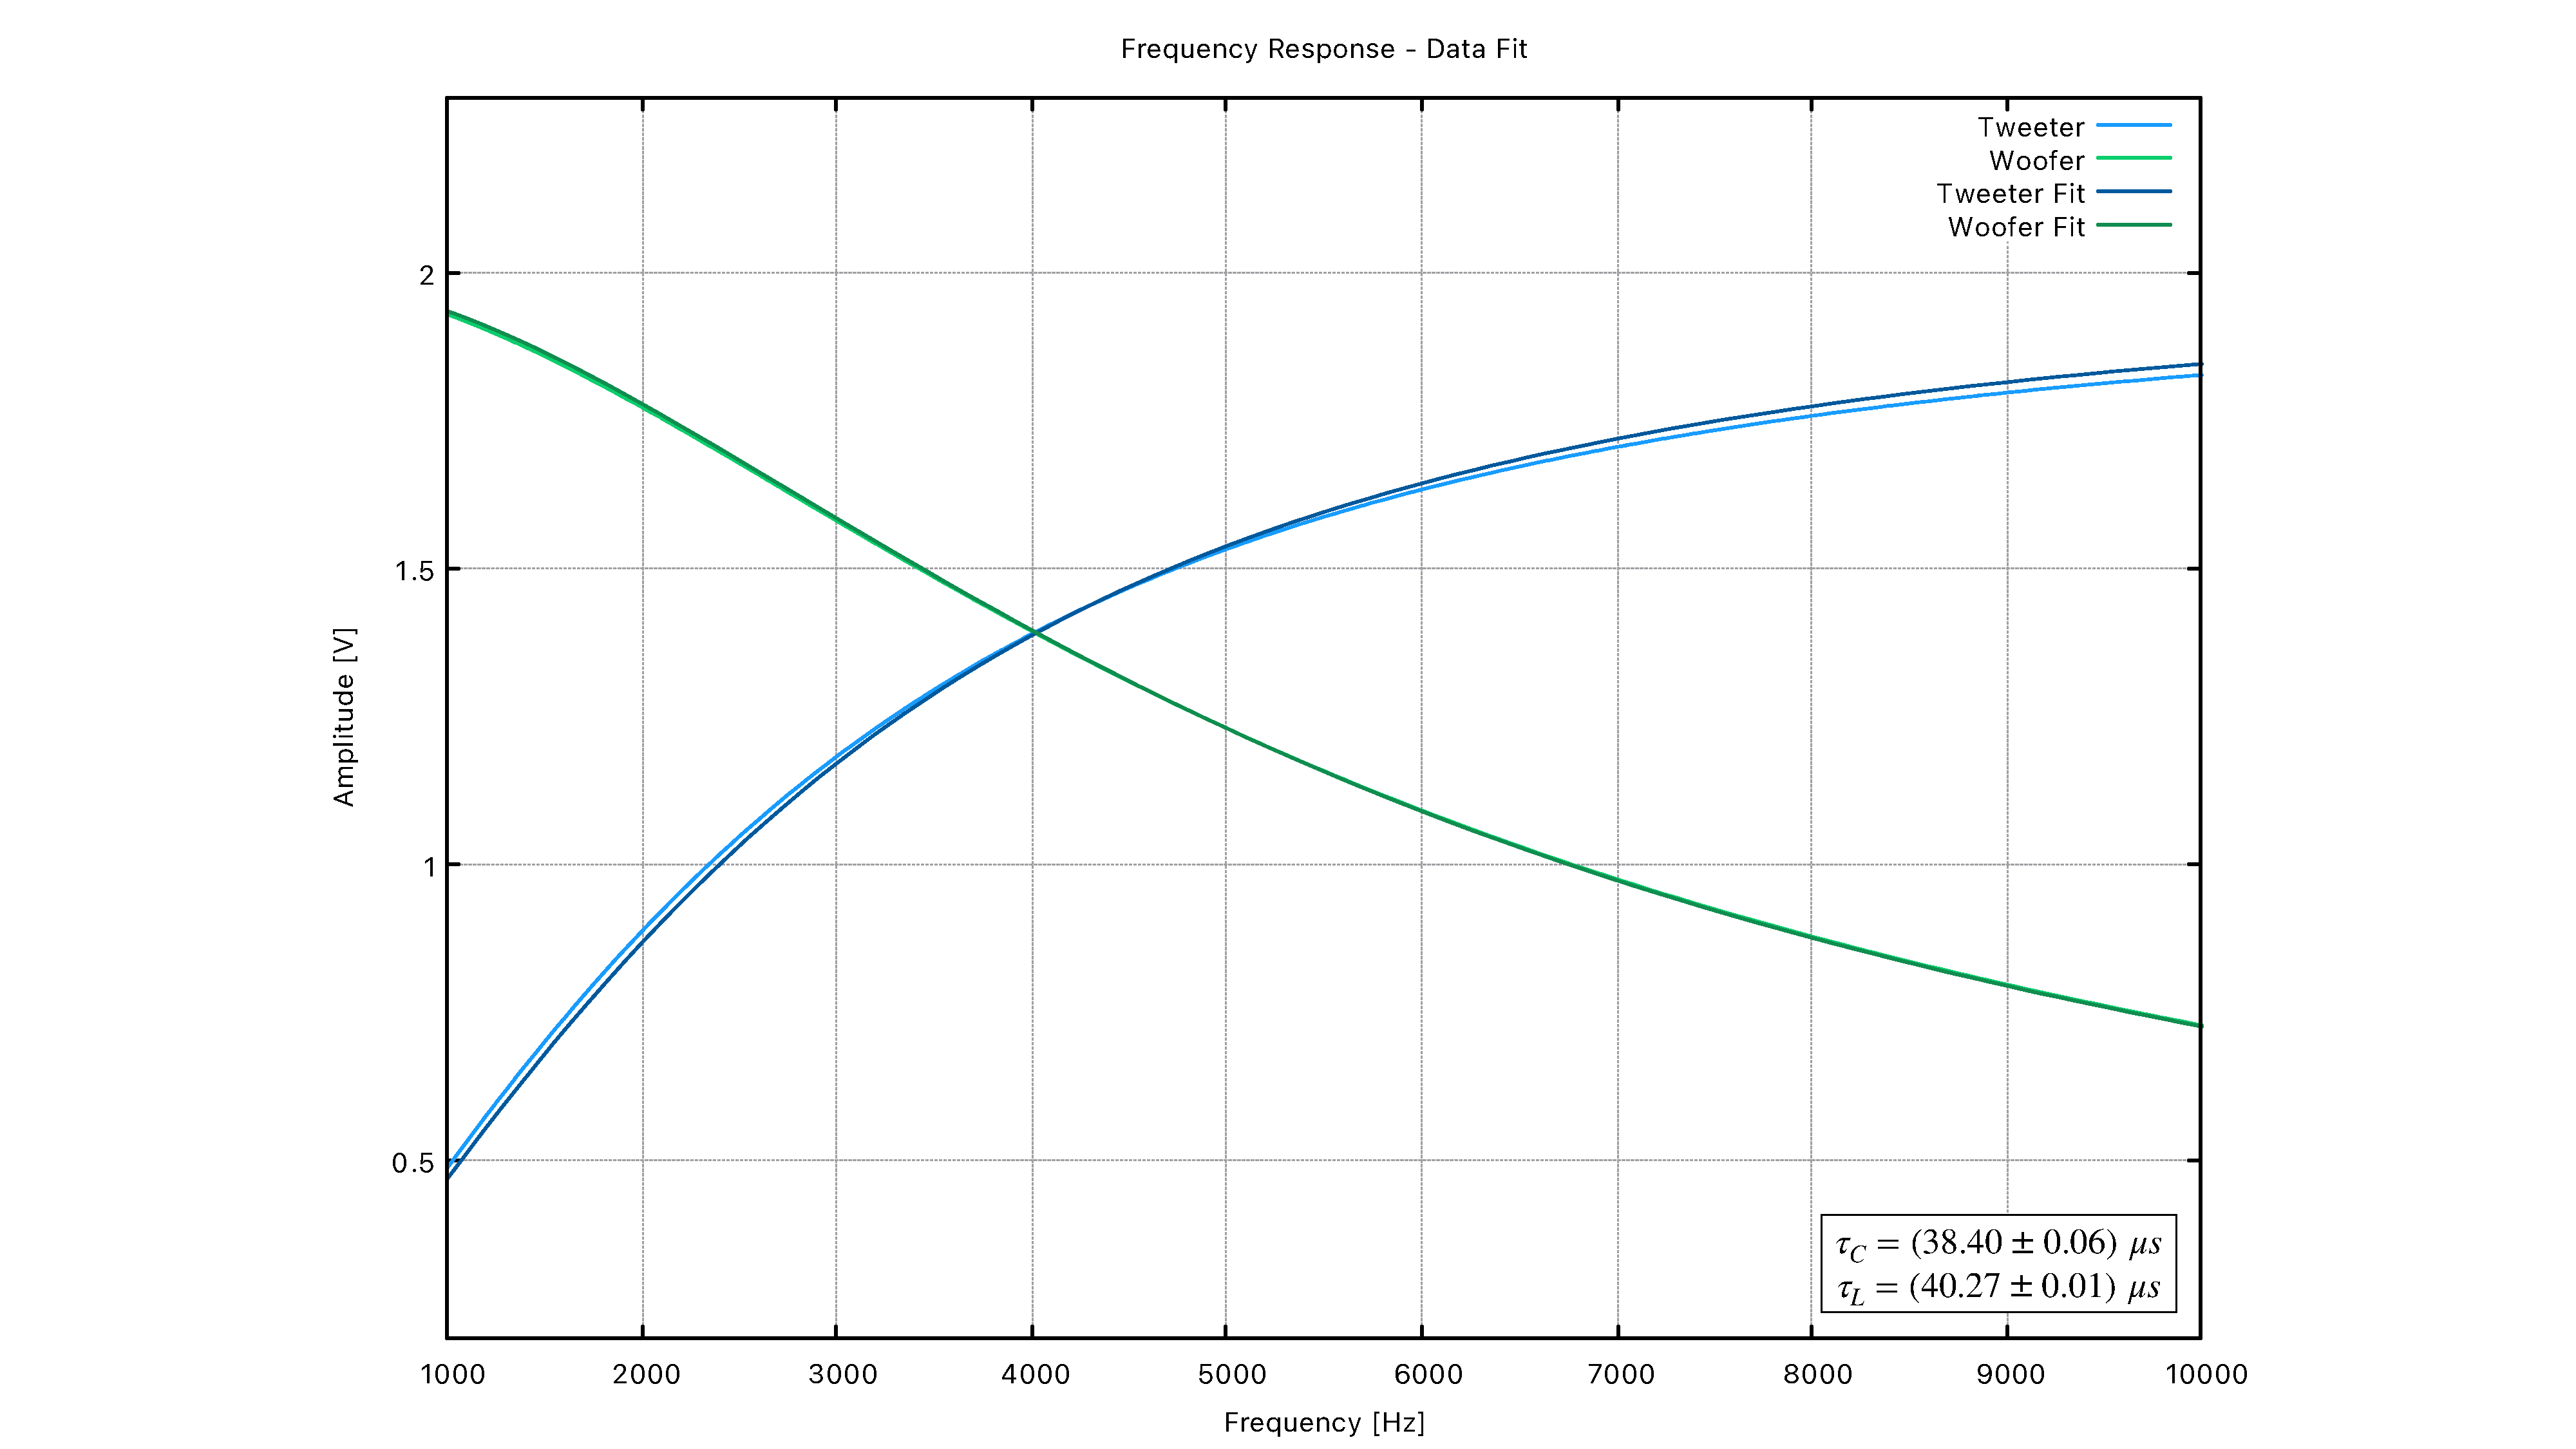
\includegraphics[width=1\linewidth]{../results/CFAmplFit.pdf}
  \caption{\textit{}}
\end{subfigure}%
\hfill
\begin{subfigure}{.5\textwidth}
  \centering
  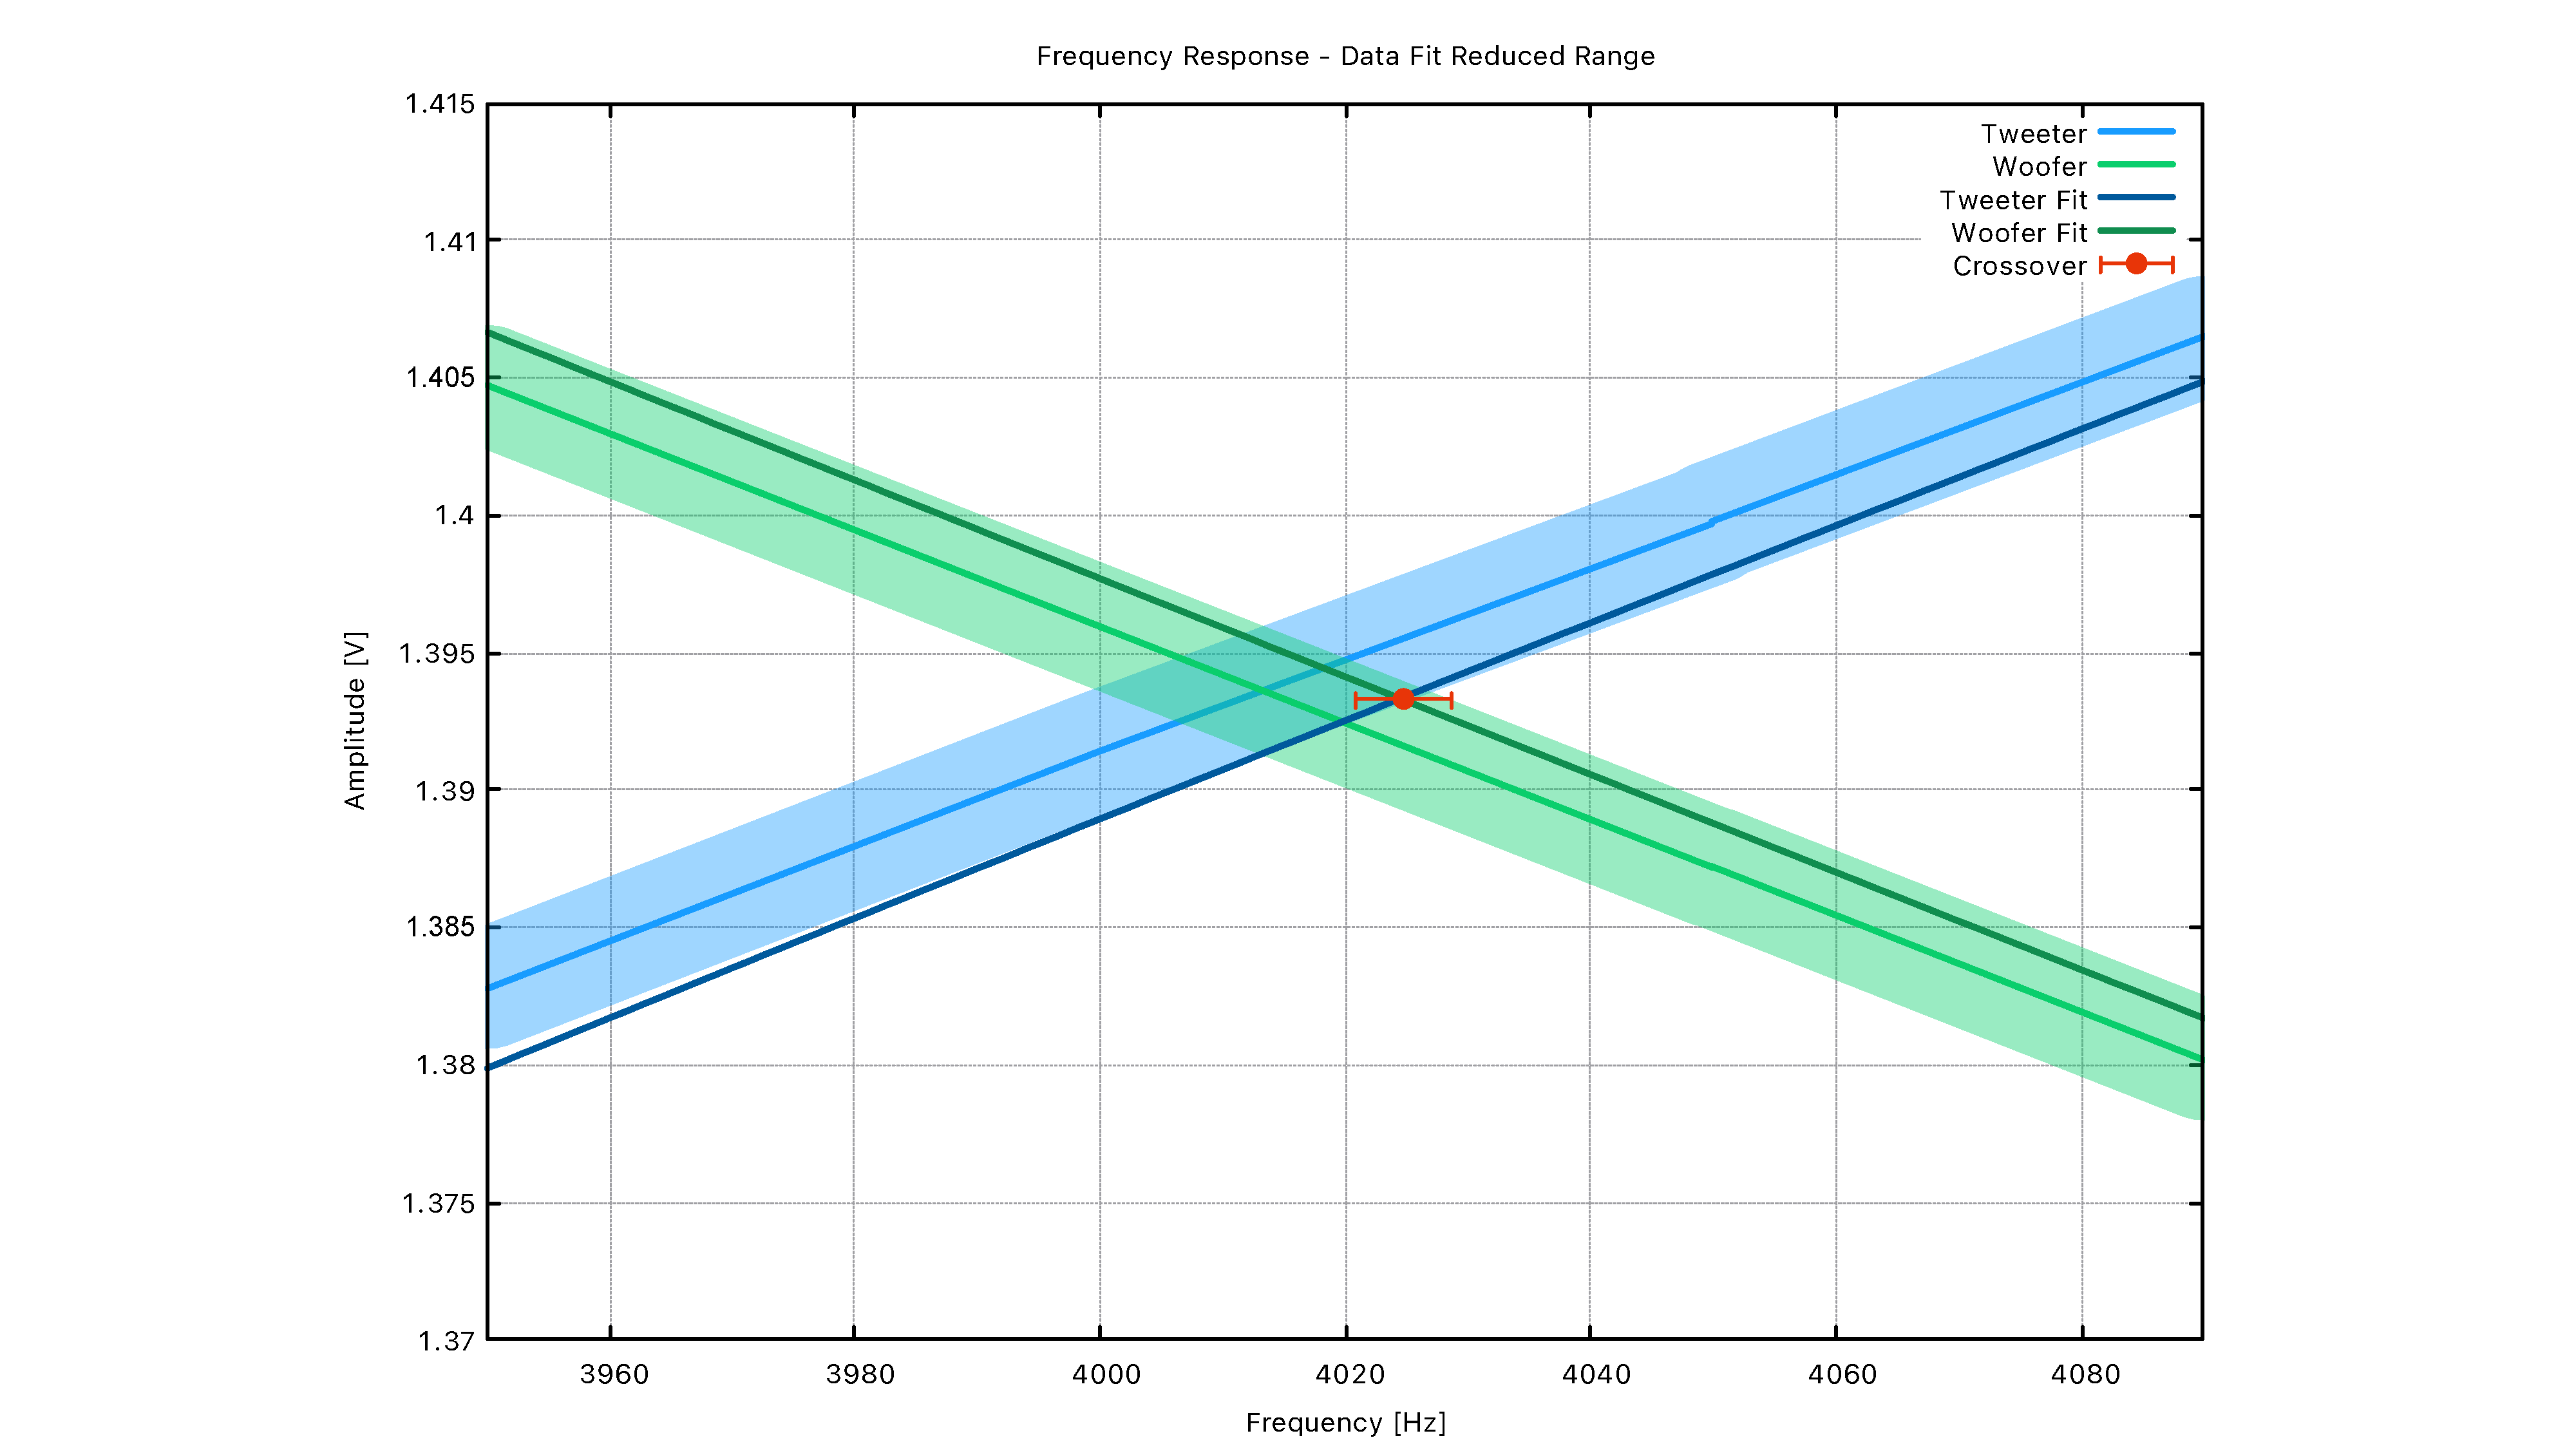
\includegraphics[width=1\linewidth]{../results/CFAmplRRFit.pdf}
  \caption{\textit{}}
\end{subfigure}
\caption{ \textit{(a) Confronto tra dati sperimentali e fit attraverso i parametri $\tau_C$ e $\tau_L$, (b) range ridotto nel quale è visibile la 
miglior stima della frequenza di crossover ricavata dai dati. }}
\end{figure}
%%%%%%%%%%%%%%%%%%%%%%%%%%%%%%%%%%%%%%%%%%

\subsection{Analisi della fase}
% Figure 5 %%%%%%%%%%%%%%%%%%%%%%%%%%%%%%%%
\begin{figure}[!ht]
  \begin{subfigure}{.5\textwidth}
    \centering
    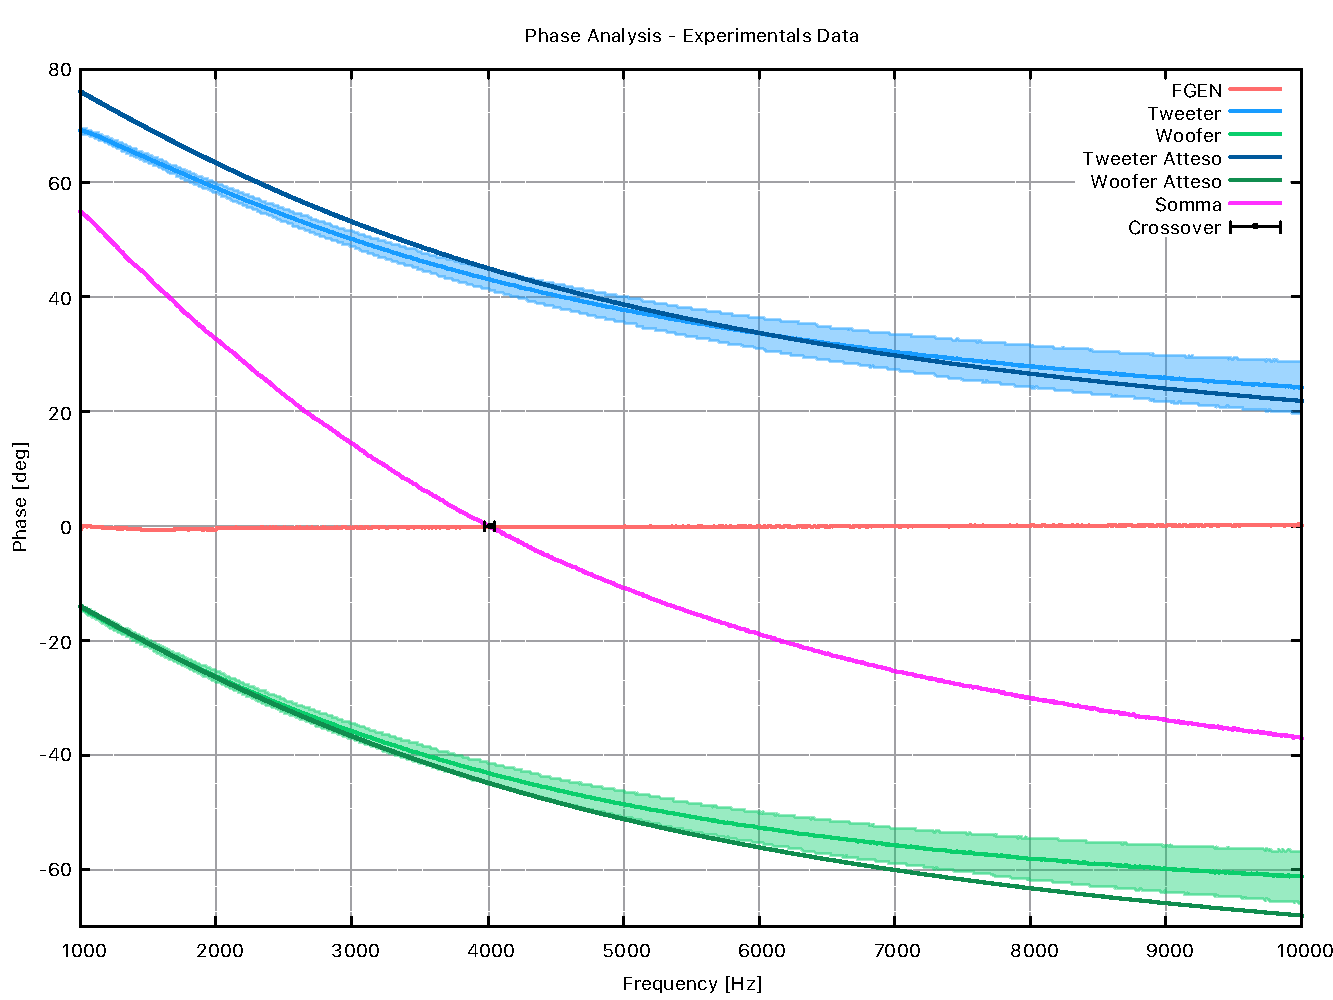
\includegraphics[width=1\linewidth]{../results/CFPhase.pdf}
    \caption{\textit{}}
  \end{subfigure}%
  \hfill
  \begin{subfigure}{.5\textwidth}
    \centering
    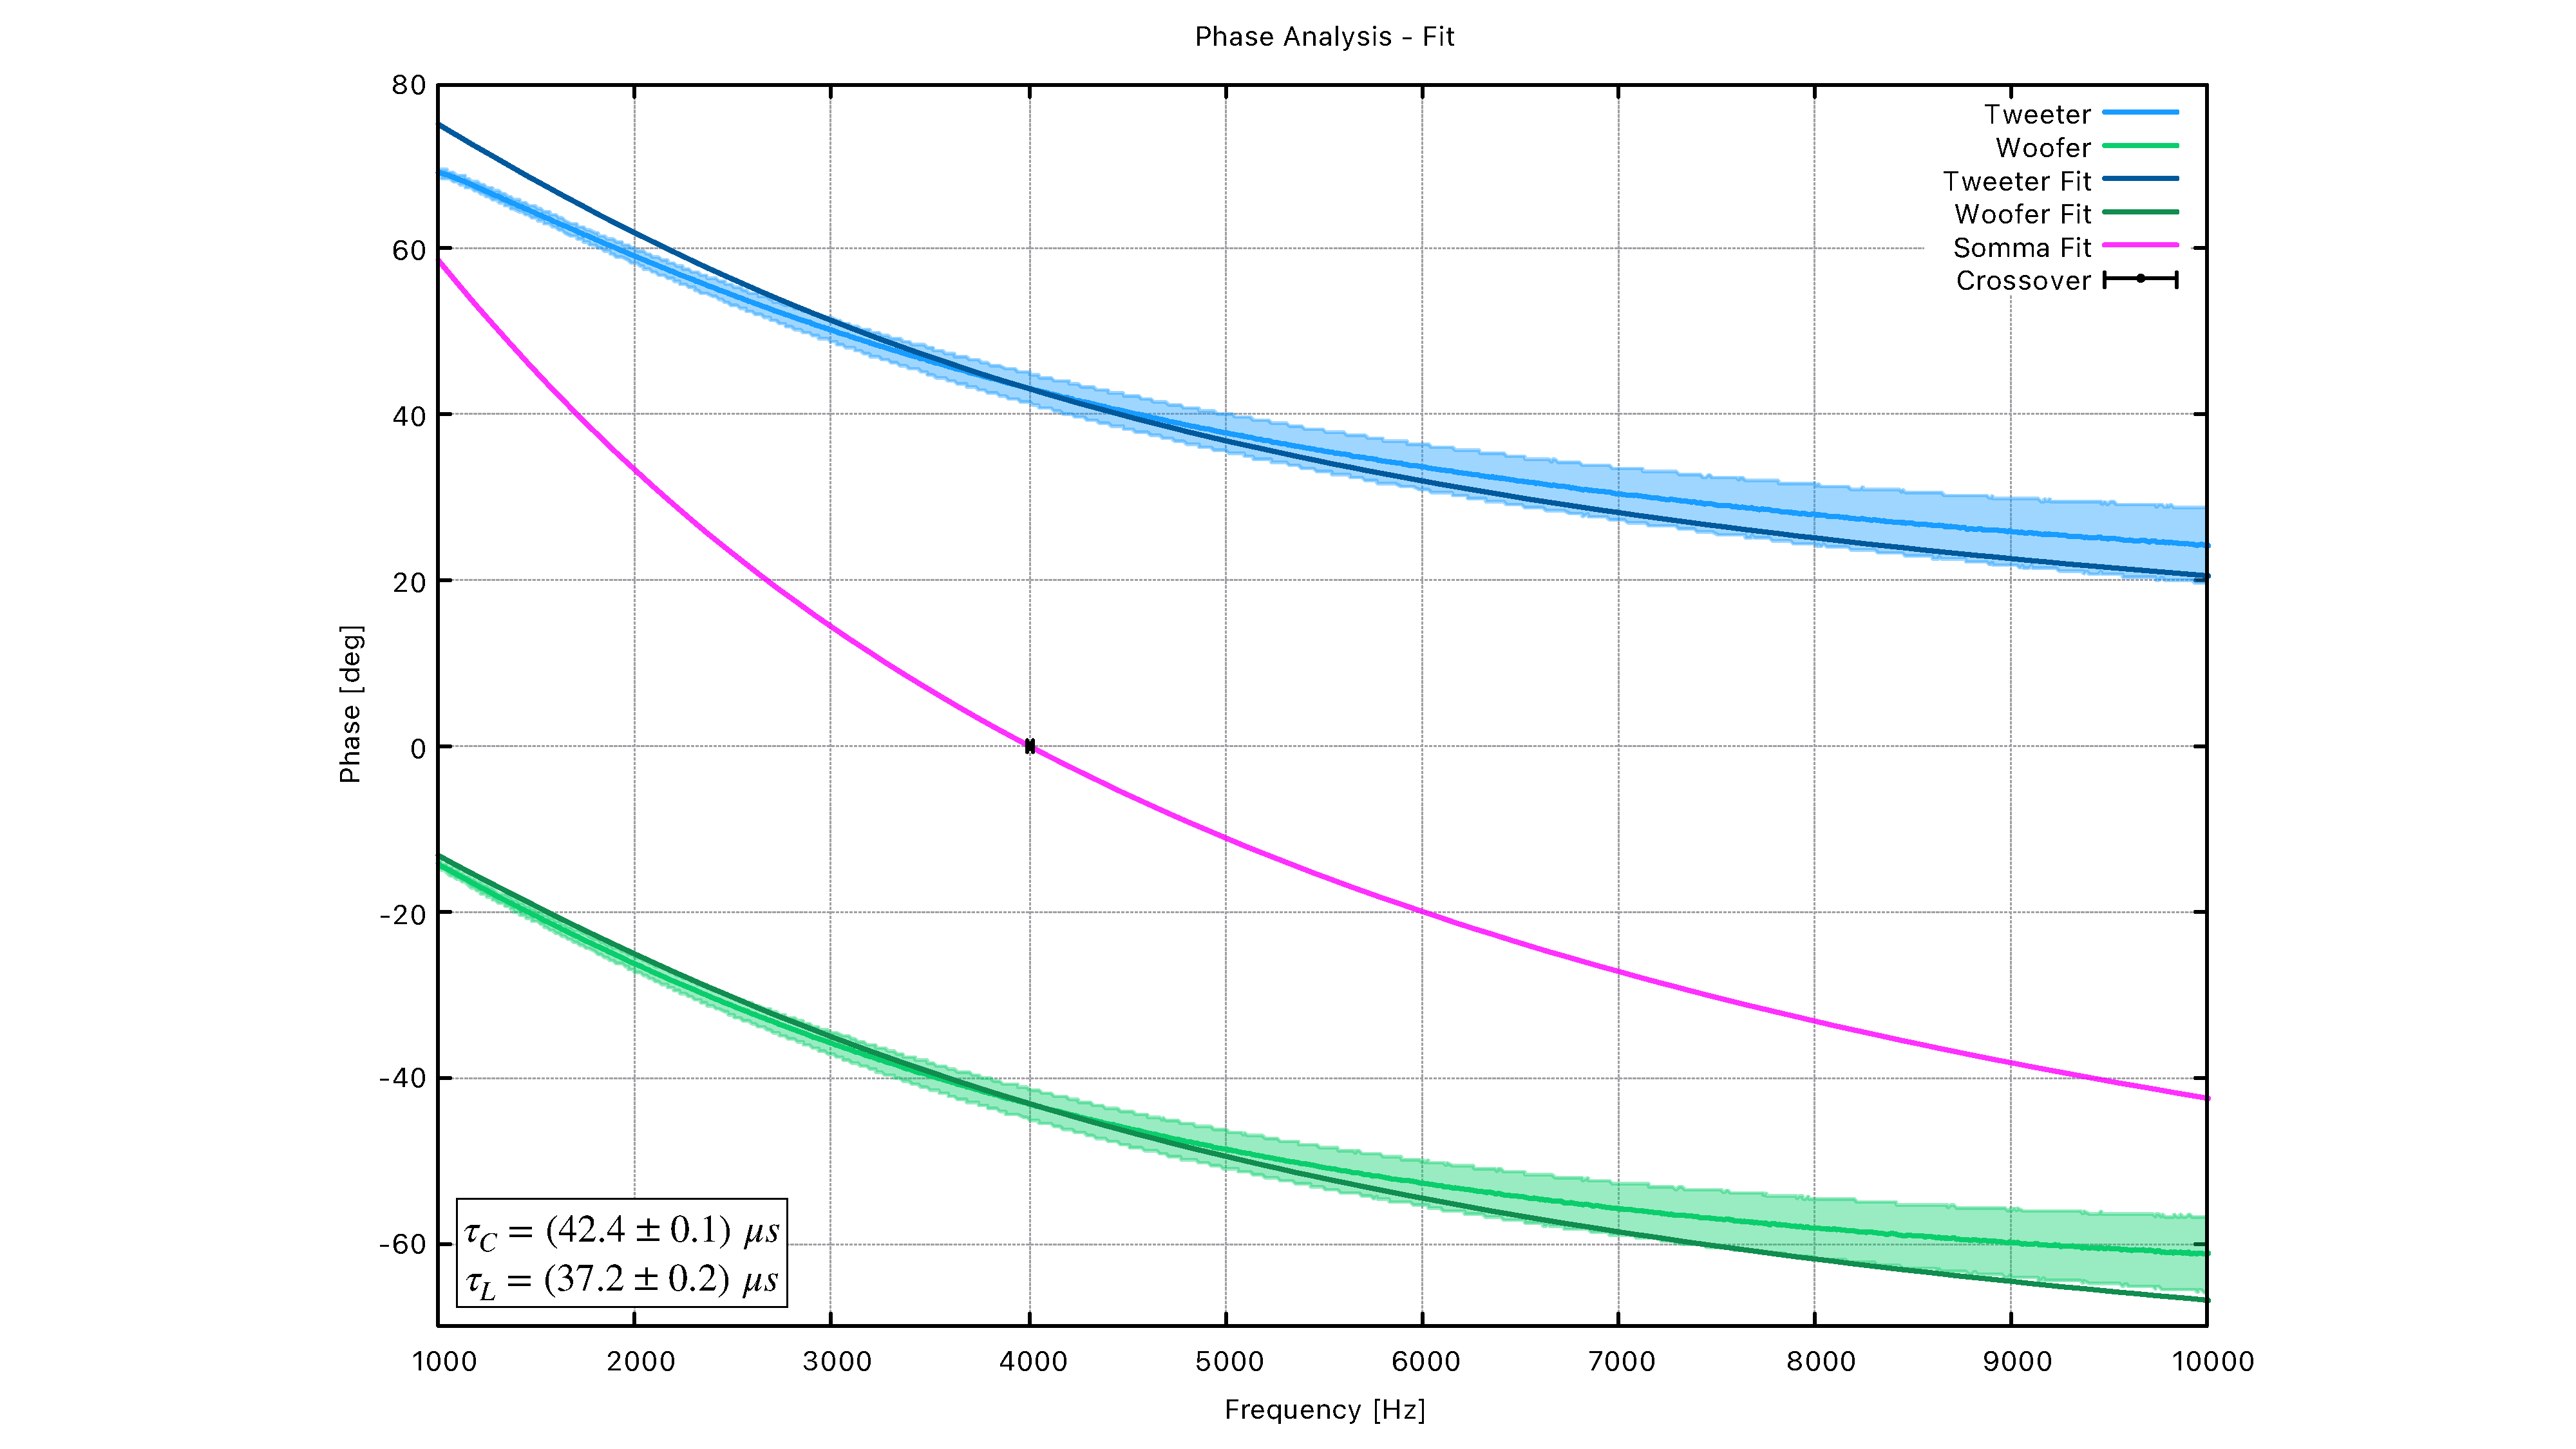
\includegraphics[width=1\linewidth]{../results/CFPhaseFit.pdf}
    \caption{\textit{}}
  \end{subfigure}
  \caption{ \textit{Analisi della fase: (a) sfasamento in funzione della frequenza rilevato nei rami del circuito 
  a confronto con le funzioni di aspettazione (equazioni (3)), sono inoltre rappresentate la somma degli sfasamenti e la frequenza 
  di crossover attesa con relativa incertezza; (b) dati sperimentali e relative curve di fit tramite i parametri $\tau_C$ e $\tau_L$, 
  si possono notare anche la somma dei fit e la miglior stima della frequenza di crossover con relativa incertezza.}}
  \end{figure}
%%%%%%%%%%%%%%%%%%%%%%%%%%%%%%%%%%%%%%%%%%
\
\\
In Fig. 5a sono rappresentati i dati sperimentali rilevati sui rami del circuito
a confronto con le curve teoriche. Ai dati sperimentali è stata associata l'incertezza 
$\delta \phi = 180 \times \nu / F_S $ ($\nu$ frequenza generata e $F_S$ frequenza di campionamento). Tale formula
costituisce una stima dell'incertezza ed è discussa in appendice. È importante precisare che 
non è conosciuto il corretto funzionamento del subVI di acquisizione dati della fase per questo motivo il metodo 
utilizzato per stimare l'incertezza è semplificato e costituisce probabilmente un sovrastima dell'errore.
Gli sfasamenti attesi seguono le seguenti espressioni:
\begin{equation}
  \phi_C(\nu) = \arctan\bigg(\frac{1}{2\pi\tau_C\nu}\bigg) \ \ \ \ \ \ \ \ \phi_C(\nu) = -\arctan(2\pi\tau_L\nu)
\end{equation}

Per determinare la miglior stima della frequenza di crossover è stato svolto un fit delle equazioni (3) sui dati sperimentali e le curve 
risultanti sono rappresentate in Fig. 5b. I parametri del fit sono:
$\tau_C=(42.41 \pm 0.11) \ \mu s$ e $\tau_L=(37.2 \pm 0.2) \ \mu s$. A questi fit sono associati i valori del chi quadrato ridotto
$\tilde{\chi^2_C}=1.45$ e $\tilde{\chi^2_L}=0.91$, entrambi i valori sono confrontabili con il valore ottimale di 1 ciò significa che 
le curve teoriche si adattano relativamente bene ai dati sperimentali.
La miglior stima della frequenza di crossover risulta essere $\nu_0 = (4007 \pm 16) \ Hz$ compatibile con quella teorica.
La stima della frequenza risulta essere molto precisa con un'incertezza percentuale del $0.4\%$, anch'essa inferiore a quella associata al valore di aspettazione.

\section{Conclusione}
L'esperienza svolta ha confermato il comportamento atteso del filtro di crossover. L'analisi dei dati relativi alla tensione 
ai capi delle resistenze $R_C$ ed $R_L$ ha evidenziato un andamento molto simile a quello previsto dalle equazioni (2) e ha portato 
ad una stima della frequenza di crossover $\nu_0 = (4024 \pm 4) \ Hz$ in accordo con quella attesa. L'analisi dello sfasamento della tensione è stato 
altrettanto soddisfacente ed ha evidenziato un andamento simile a ciò che ci si aspettava dalle equazioni (3). La stima della 
frequenza di crossover è stata $\nu_0 = (4007 \pm 16) \ Hz$ in accordo con quella attesa $\nu_0 = (4021 \pm 40) \ Hz$. Il test d'ipotesi svolto 
in ambedue le analisi ha portato a valori del chi quadrato ridotto relativamente lontani dal valore ottimale di 1 (soprattutto nell'analisi della tensione). Questa leggera discordanza 
può essere attribuita ad una stima sbagliata dell'incertezza associata a fase ed ampiezza (probabilmente sovrastimate).

\subsection*{Appendice}
\paragraph{1} 
Per ricavare le equazioni (1), (2), e (3) facendo riferimento alla Fig. 1 procediamo con la legge di Kirchhoff per la maglia 
dell'induttore:
$$
  \vec{V}=(R_{IL}+j\omega L)\vec{I_L} + \vec{V_L}=\frac{R_{IL}+j\omega L}{R_{L}+R_{IL}+j\omega L}\vec{V}+\vec{V_L}
$$ $j$ unità immaginaria e $\omega = 2\pi \nu$ pulsazione del segnale. Isolando $\vec{V_L}$ di ha:
$$
\vec{V_L} = \frac{R_L}{R_L+R_{IL}+j\omega L}\vec{V}=\frac{r_L}{1+j\omega \tau_L} \vec{V}
$$ con $r_L = \nicefrac{R_L}{(R_L+R_{IL})}$ e $\tau_L=\nicefrac{L}{(R_L+R_{IL})}$.
Nella maglia del condensatore procedendo nella stesso modo si ha:
$$
\vec{V_C} = \frac{R_C}{R_C+R_{IC}+\frac{1}{j \omega C}}\vec{V}=\frac{r_C}{1+\frac{1}{j\omega \tau_C}} \vec{V}
$$ con $r_C = \nicefrac{R_C}{(R_C+R_{IC})}$ e $\tau_C=C(R_C+R_{IC})$. In questo modo ho la relazione
tra tensione in entrata e quella sui rami del circuito. Calcolando il modulo e la fase ho rispettivamente 
le equazioni (2) e (3). Per avere l'equazione (1) si può procedere eguagliando i moduli delle tensioni sui rami, 
ricordando che per costruzione $r_C=r_L$ si ha che:
$$
\frac{r_L V}{\sqrt{1+(2 \pi \tau_L \nu_0)^2}}=\frac{r_C V}{\sqrt{1+\frac{1}{(2 \pi \tau_C \nu_0)^2}}} \rightarrow \nu_0 = \frac{1}{2\pi \sqrt{\tau_C\tau_L}}
$$
\paragraph{2} 
L'incertezza sulla misura della fase è stata stimata usando una possibile espressione per lo sfasamento tra due onde sinusoidali con la stessa frequenza:
$\phi=360\times\Delta t/T$ ($\Delta t$ distanza temporale tra picchi delle due onde e $T=1/\nu$). Assumendo $\delta t=1/(2F_S)$ si ha $\delta(\Delta t) = \delta t = 1/(2F_S)$ 
quindi $\delta\phi =180\times \nu/F_S$. 
\end{document}